%%%%%%%%%%%%%%%%%%%%%%%%%%%%%%%%%%%%%%%%%
% Thin Sectioned Essay
% LaTeX Template
% Version 1.0 (3/8/13)
%
% This template has been downloaded from:
% http://www.LaTeXTemplates.com
%
% Original Author:
% Nicolas Diaz (nsdiaz@uc.cl) with extensive modifications by:
% Vel (vel@latextemplates.com)
%
% License:
% CC BY-NC-SA 3.0 (http://creativecommons.org/licenses/by-nc-sa/3.0/)
%
%%%%%%%%%%%%%%%%%%%%%%%%%%%%%%%%%%%%%%%%%

%----------------------------------------------------------------------------------------
%	PACKAGES AND OTHER DOCUMENT CONFIGURATIONS
%----------------------------------------------------------------------------------------

\documentclass[a4paper, 11pt]{article} % Font size (can be 10pt, 11pt or 12pt) and paper size (remove a4paper for US letter paper)
\usepackage[ruled]{algorithm2e}
\usepackage[protrusion=true,expansion=true]{microtype} % Better typography
\usepackage{graphicx} % Required for including pictures
\usepackage{wrapfig} % Allows in-line images
\usepackage{amsmath, amsfonts}
\usepackage{hyperref}
\usepackage{subfigure}
\usepackage{booktabs}
\usepackage{makeidx}
\usepackage[numbers]{natbib}
\usepackage[usenames,dvipsnames]{color}


\newcommand{\stnote}[1]{\textcolor{Blue}{\textbf{ST: #1}}}
\newcommand{\menote}[1]{\textcolor{Red}{\textbf{ME: #1}}}

\usepackage{mathpazo} % Use the Palatino font
\usepackage[T1]{fontenc} % Required for accented characters
\linespread{1.05} % Change line spacing here, Palatino benefits from a slight increase by default
\makeatletter
\renewcommand\@biblabel[1]{\textbf{#1.}} % Change the square brackets for each bibliography item from '[1]' to '1.'
\renewcommand{\@listI}{\itemsep=0pt} % Reduce the space between items in the itemize and enumerate environments and the bibliography

\renewcommand{\maketitle}{ % Customize the title - do not edit title and author name here, see the TITLE block below
\begin{flushright} % Right align
{\LARGE\@title} % Increase the font size of the title

\vspace{50pt} % Some vertical space between the title and author name

{\large\@author} % Author name
\\\@date % Date

\vspace{40pt} % Some vertical space between the author block and abstract
\end{flushright}
}

%----------------------------------------------------------------------------------------
%	TITLE
%----------------------------------------------------------------------------------------

\title{\textbf{Incrementally Interpreting Multimodal Referring Expressions in Real Time}} % Subtitle

\author{\textsc{Miles Eldon}\\ % Author
\textsc{Professor Stefanie Tellex} (Reader and Advisor)\\
{\textsc{Professor Michael Littman} (Second Reader)}
\\{\textit{Brown University}}} % Institution

\date{\today} % Date

%----------------------------------------------------------------------------------------
\begin{document}

\maketitle % Print the title section
\newpage
\tableofcontents
\newpage
\section{Introduction}
Robots have long been a great asset in controlled settings, such as factories, yet remain unable to make the crucial leap into daily life, interacting with humans. In order for humans and robots to collaborate in complex tasks, robots must be able to understand people's references to objects in the real world. For example, a robotic assistant might be asked to fetch a tool in a factory setting, or medicine in a hospital setting, or ingredients in a kitchen. Figure~\ref{fig:example} shows Baxter handing a bowl to a chef. To refer to objects, people use a fluid combination of speech, gesture, eye gaze, and a variety of other body language. People provide these referring expressions continiously, and can change rapidly based on new information from the agent they are instructing or their perception of the environment. This new information from a partner can be in the form of confirming signals, such as nodding of the head, or requests for clarification, such as looking confused or asking questions.~\citet{clark96} refers to this back and forth of instruction and clarification or confirmation as a \textit{joint activity}, used to assist in collaborative tasks by creating common ground and reducing uncertainty.


Responding quickly and accurately are critical for a truly interactive robotic assistant in everyday life. By continously interpreting human referring expressions, a robotic assistant can not only respond quickly, but also incorporate the relative timing of gestures and speech in a natural manner. Continous interpretation make interactions more rapid and fluid, and also enable a robot to provide affirming or clarifying feedback in a time frame that is reasonable. This rapid feedback makes these human robot interactions more meaningful by quickly leading to mutual understanding, either with both agents proceeding with their own tasks, or with the human clarifying a request for the robot, rather than necessitating a different system of the human confirming that a request was understood.

\begin{figure}[h]
\centering
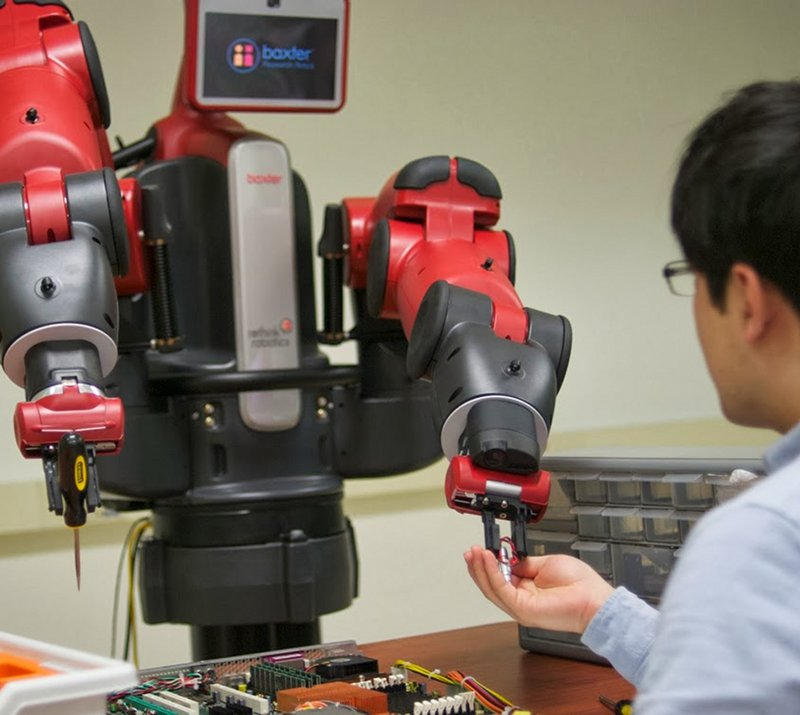
\includegraphics[width=0.3\linewidth]{images/baxter_scene_cropped.jpg}
\caption{Robots that collaborate with people need to understand their
  references to objects in the environment.  For example, if a person
  asks for a tool using language and gesture, the robot needs to
  interpret the person's reference in order to pick up the correct
  tool.\label{fig:example}}
\end{figure}

Despite the importance of a system capable of real-time response to multimodal input, existing models approaches fail to meet this high bar. Several systems focus on single modalities, which are insufficient to handle complicated interactions, such as ambigious phrases accompanied by gestures or vice versa~\citep{tellex11, kollar10}. Approaches that have incorporated multiple sources have failed to do so in an online manner, relying on batch interpretation, which is not fast enough for systems that need to respond immediately~\citep{matuszek14}. These approaches preclude rapid reaction, clarifying feedback, and the level of interpretation necessiated by human referring expressions.

To provide a foundation for these capabilities, we propose a Bayes' Filter to interpret information from language and gesture~\citep{thrun08}. Our framework relies on a factored observation probability that fuses information from language and gesture in real time to continuously estimate the object a human user is referencing. We initially demonstrate our model in simulation, and then perform user studies with our system running on a RGB-D corpus of untrained users referencing objects on a table. The results show that our model quickly and effectively fuses multimodal information in real time to continously estimate the object being referenced. Additionally, we demonstrate a robot that uses our model to provide feedback in the form of facial expressions, pointing, and handing the user the object referenced in real time by interepreting gesture and language.

\begin{figure*}
\centering
\subfigure[Ambiguous gesture.\label{fig:confused}]{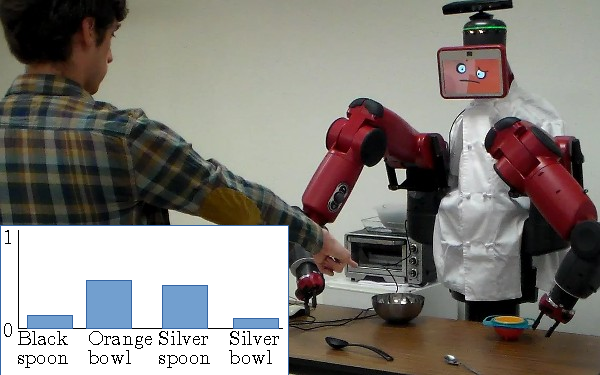
\includegraphics[width=0.49\linewidth]{images/cartoon1.pdf}}
\subfigure[Clarification with language.\label{fig:clarified}]{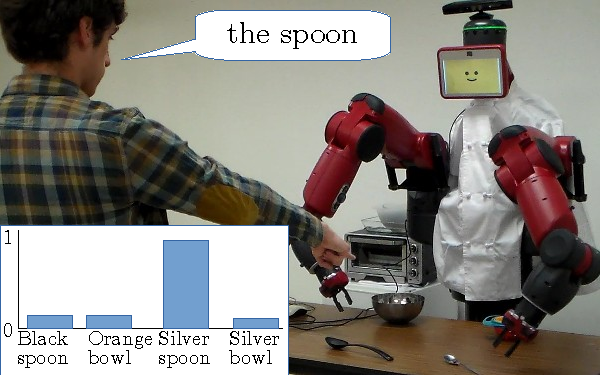
\includegraphics[width=0.49\linewidth]{images/cartoon2.pdf}}
\caption{After an ambiguous gesture, the model has a uniform
  distribution between two objects (a).  The robot responds by
  indicating confusion.  Clarification with language causes a
  probabilistic update leaving the model highly confident it has
  inferred the correct object (b).  The robot responds by smiling and
  pointing to the correct object. \label{fig:cartoon}}
\end{figure*}

\section{Related Work}
~\citep{clark96} proposed that conversation is a \textit{joint activity}, a coordinated, collaboraitve process in which the two participants establish \textit{common ground}. Common ground refers to the process by which each participant establishs an understanding about the beliefs of the other. In order to establish common ground, people use various forms of feedback, ranging from head nods to looks of confusion to explicit clarifying questions. These forms of feedback allows the participants to iteratively establish common ground through instruction and clarification as time progresses. Our Bayes' Filter approach provides a foundation for producing this feedback with a robot, which has the ability to increase robustness and reduce rate of error in human-robot communication through the establishment of common ground during interactions.

A large body of research focuses on language understanding for robots, ignoring information, but fails to account for the continuous nature of language, requiring full sentences or some other form of batching before interpretation can take place~\citep{macmahon06, dzifcak09, kollar10, matuszek12}. While this batching can help improve accuracy, the delays it imposes are unreasonable for a real time system. Our approach, in contrast, incorporates each word as it is processed during speech recognition, integrating it over time and fusing it with body language. In a similar vein as our research, \citet{guadarrama14} interprets open-domain references to objects, but still fails to include gesture, precluding natural non-verbal references. \citet{cantrell10} provides a framework for incrementally interpreting language, but neither includes language nor corpus based results. Our approach draws several ideas from each of these, but focuses on a more robust system of continuous understanding and interpretation.

Many other approaches for command interpretation depend on command words such as ``follow'' or ``stop''~\citep{waldherr00, marge11}. This type of system goes directly against what is desired, which is that an untrained user could interact with the system in whatever way felt most natural, rather than enforcing some small set of keywords that trigger specific behavior. This type of system removes the ability to make a robotic assistant to appear human in it's actions and reactions, and also ignores the importance of body language in interactions, as well as continuous interpretation of language.

\citet{matuszek14} presented work that falls closest to ours; a multimodal framework for interpreting unscripted references to tabletop objects using language and gesture, providing an accuracy rate comparable to the accuracy our system demonstrates in correctly indentifying the referenced object. However, this system relies on interpretation of batched data, failing to operate in real time, strictly limiting it in comparison to our continuous Bayes' Filter approach.

Partially Observable Markov Decision Process approaches to dialogue interpretation have been extended to incorporate gesture and noise models, similiar to our approach~\citep{young13, young10} . We have begun exploring similar methods of generating robot response, leading to informative feedback from a robotic assistant. \citet{dragan13} created a system to enable a robot to create gestures designed to strike a balance between legibility and predictibility. While we have explored the research in creating feedback, we have mostly focused on interpreting these gestures from humans, rather than generating them. Our long-term aim is to combine the understanding we have created with these systems to produce feedback, allowing for the rapid creation of common ground between a robotic assistant and a human user.
\section{Technical Approach}
Our aim is to estimate a distribution over which object a human user is referencing given language and body pose inputs. We frame this problem as a Bayes' Filter~\citep{thrun08}, where the \textit{hidden} state $x \in \mathcal{X}$ is the object in the scene the person is currently referencing. The robot observes the speech and gesture $z \in \mathcal{Z}$ at each timestep $t$ and continuously estimates a distribution over $x_t$, as shown in Figure~\ref{fig:model}. This model requires access to a transisition function specifying $p(x_t | x_{t-1})$ and an observation function specifying $p(z_t | x_t)$. Part of our model involves the development of these functions.

\begin{figure}[h]
\centering
\fbox{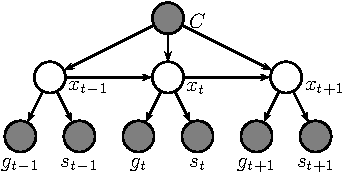
\includegraphics{images/bigram-crop.pdf}}
\caption{Graphical model for our approach with each observation factored into gesture ($g$) and speech ($s$). $C$ is the overall contextual information.\label{fig:model}}
\end{figure}

Formally, we wish to calculate:
\begin{align}
p(x_t | z_0, \dots, z_t)
\end{align}

To estimate this distribution, we perform alternating time and measurement updates. The time update incorporates the hidden state transitions using the previous state estimate and knowledge of the state transitions:
\begin{align}
p(x_t | z_{0:t-1}) = \int_{x_{t-1} \in \mathcal{X}} p(x_t|x_{t-1})\times p(x_{t-1} | z_{0:t-1}) \text{d}x_{t-1}
\end{align}

The measurement update combines the previous belief with the newest observation to update each belief state: 
\begin{align}
p(x_t |z_{0:t}) = \frac{p(z_t | x_t) \times p(x_t | z_{0:t-1})}{p(z_t | z_{0:t-1})} \\\propto p(z_t | x_t) \times p(x_t | z_{0:t-1})
\end{align}

Once normalized, this gives us an easily calculable, accurate estimation of the users state at each time step.
\subsection{Transition Model}
We assume that a person is likely to continue referring to the same
object, and so has a large probability $c$ of remaining in the state

\begin{align}
p(x_t | x_{t-1}) = \left\{  \begin{array}{ll}
c&\mbox{if } x_t = x_{t-1}\\
1-\frac{c}{|X|-1}&\mbox{otherwise}
\end{array}\right.
\end{align}

This assumption means that the robot's certainty slowly decays in the absence of meaningful observations, convergine to a uniform distribution. This enables our framework to find a balance between integrating past information and incorporating new, contrary information to switch the most likely estimated state.
\subsection{Observation Model}
We assume access to an observation model of the form:
\begin{align}
p(z_t | x_t)
\end{align}

Observations consist of a tuple consisting of a person's actions,
$\langle l, r, h, s\rangle $ (shown in Figure~\ref{fig:labeled_obs}) where:
\begin{itemize}
    \item $l$ represents a vector from the observed origin ($l_o$) to the point ($l_v$) of the left arm.
    \item $r$ represents a vector from the observed origin ($r_o$) to the point ($r_v$) of the right arm.
    \item $h$ represents a vector from the observed origin ($h_o$) to the point ($h_v$) of the head. This is the angle of the head transformed into a unit length vector.
    \item $s$ represents the observed speech from the user,
          consisting of a list of words.
    \end{itemize}

\begin{figure}[h]
\centering
\fbox{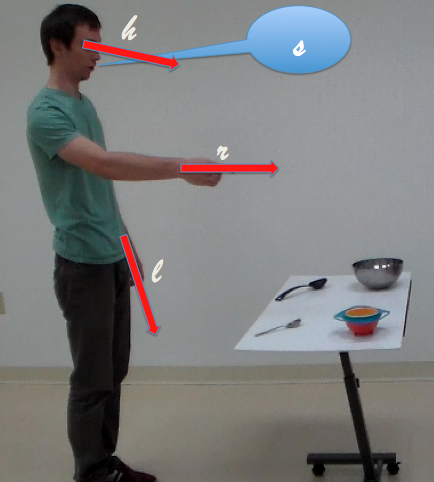
\includegraphics[scale=0.5]{images/labeled_obs.png}}
\caption{An image from our corpus with the components of observation labeled.\label{fig:labeled_obs}}
\end{figure}
Formally, we have:
\begin{align}
p(z_t | x_t) &= p(l, r, h, s | x_t)\\
\intertext{We factor assuming that each modality is conditionally independent of the others given the state (the true object that the person is referencing):}
p(z_t | x_t) &= p(l | x_t) \times p(r | x_t) \times p(h | x_t) \times p(s | x_t)
\end{align}
\subsubsection{Modeling Gesture}
We track body pose using the NITE skeleton tracker~\citep{openni}. We use this skeletal pose information to extract the 3D vector representing each forearm and the angle of the head (a unit length vector computed based on the observed rotation of the head). We then project the forearm gestures such that each arm vector actually originates in the wrist, as shown in Figure~\ref{fig:labeled_obs}. These three vectors comprise our deictic gestures.

To convert each vector observation $v$ into a probability for each object we need to compute $p(v | x_t)$. Since $v$ is composed of an origin $o$ and a point $p_1$, we simply take the center of mass of the object $x_t$, which we will call $p_2$. Next, we define a function $\mbox{A}(o, p_1, p_2)$ to calculate the angle between $p_1$ and $p_2$ using origin $o$. With this angle, we then calculate the density of a Gaussian  distribution $\mathcal{N}$ with zero mean and variance $\sigma$ to convert the angle into a probability. Formally, this gives us:
\begin{align}
p(l | x_t) \propto \mathcal{N}(\mu_l=0, \sigma_l)[A(l_o, l_v, x_t)]\\
p(r | x_t) \propto \mathcal{N}(\mu_r=0, \sigma_r)[A(r_o, r_v, x_t)]\\
p(h | x_t) \propto \mathcal{N}(\mu_h=0, \sigma_h)[A(h_o, h_v, x_t)]
\end{align}
\subsubsection{Modeling Speech}
\subsubsection{Null Words and Gestures}
\subsection{Model Parameters}
\subsection{Assumptions}
\section{Evaluation}
\subsection{Simulation Results}
\subsection{User Studies}
\subsection{Sources of Error}
\section{Future Work}
\section{Conclusion}
\end{document}